\section{Introduction}
    \label{sec:intro}

    Le projet décrit dans ce rapport consiste à développer un logiciel d'analyse informatique des ADTrees\footnote{Abréviation d'\og Attack-Defense Trees \fg{}, ou \og Arbres d'Attaque et de Défense\fg{} en français}. Ce logiciel, baptisé Glasir et dont le logo est visible sur la {\sc Figure}~\ref{fig:glasir}, intègrera ADTool~\cite{ADTool}, un outil d'édition d'ADTrees déjà existant. ADTool sera utilisé dans Glasir pour l'affichage, la création et l'édition des ADTrees, et subira quelques modifications destinées à améliorer son ergonomie. Glasir, pour sa part, fournira les fonctionnalités d'analyse suivantes :

    \begin{itemize}
    	\item l'Éditeur de fonctions, qui permetra d'étendre le nombre de paramètres d'analyse qu'offre ADTool ;
    	\item le Filtre, qui aidera l'utilisateur à ôter de l'ADTree les nœuds aux valuations hors d'un intervalle défini ;
    	\item l'Optimiseur, qui sélectionnera le meilleur chemin dans l'ADTree selon une certaine valuation.
    \end{itemize} 

    Trois rapports ont déjà été rédigés dans le cadre de ce projet : celui de pré-étude~\cite{pre_etude}, celui de spécifications fonctionnelles~\cite{spec_fonc} et celui de planification~\cite{planif}. Ces derniers ont permis de mieux définir les objectifs du logiciel ainsi que l'organisation de son implémentation. En décembre, nous avons rendu compte de l'état de notre travail par le biais de deux soutenances : l'une consacrée à la gestion du projet et à sa planification, et l'autre décrivant le projet de façon générale. 

    Le présent rapport de conception logicielle a pour but de détailler l'architecture de Glasir. Ce rapport commencera donc par illustrer grossièrement cette architecture à l'aide d'un prototype d'interface et d'un diagramme de cas d'utilisation, afin de montrer les actions accessibles à l'utilisateur. Puis un diagramme de classes et des diagrammes de séquence permettront de détailler beaucoup plus précisément l'agencement interne du logiciel. Une partie sera ensuite consacrée aux améliorations prévues pour ADTool, puis les limites d'utilisation de Glasir seront évoquées. Enfin, un bref résumé du planning et de l'organisation prévue sera effectué.

    \vspace{4mm}

    \begin{figure}[H]
        \centering
        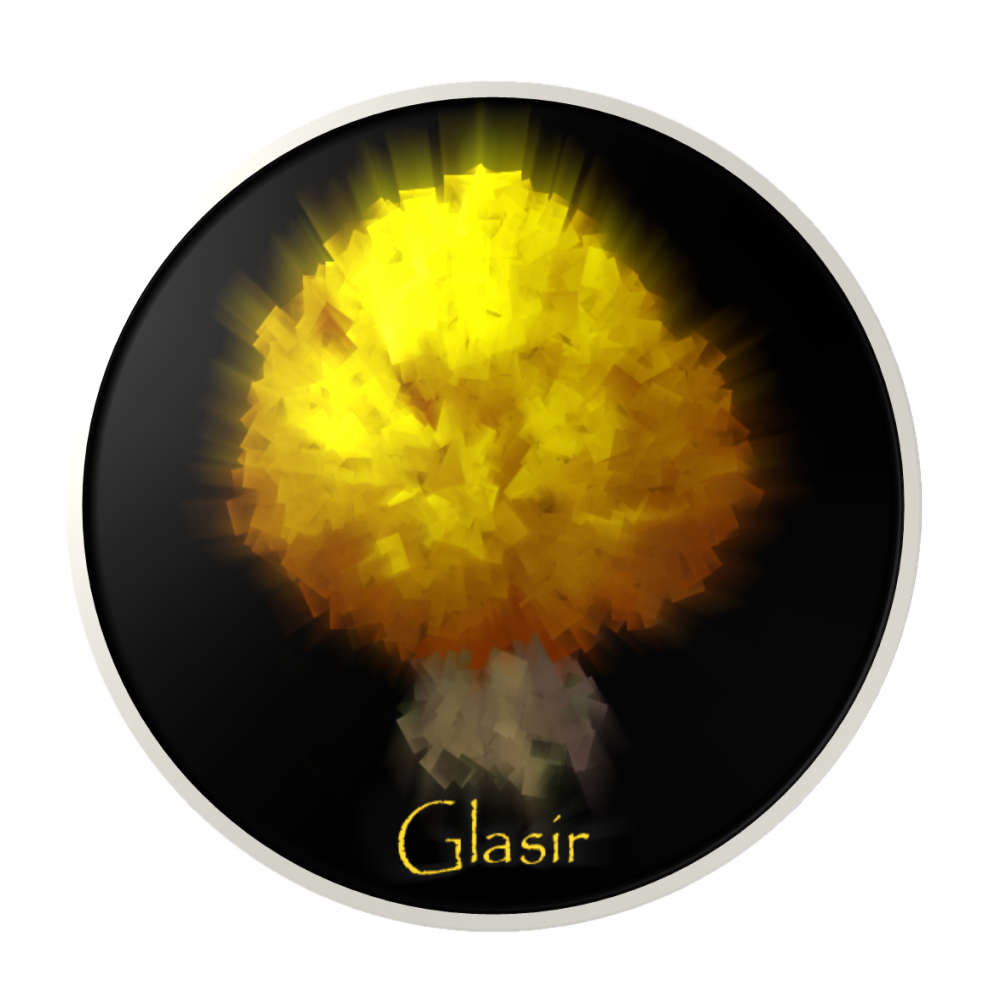
\includegraphics[height=0.5\textwidth]{figure/glasir.png}
        \caption{Logo du logiciel Glasir.}
        \label{fig:glasir}
    \end{figure}
